\documentclass[10pt,conference]{IEEEtran}

\usepackage{graphicx}
\usepackage{booktabs}
\usepackage{url}
\usepackage{hyperref}
\hypersetup{pdftitle={},pdfauthor={},pdfcreator={},pdfproducer={}}
\emergencystretch=3em

% --- ICSE 2027 is double-anonymous: do not include author identities in the PDF ---
\title{From Parsing to Adjudication: A Reproducible Protocol-by-Artifacts Framework for AI Agents}

\begin{document}
\maketitle

\begin{abstract}
Interoperability claims in AI agent ecosystems are often validated through
textual interpretation and permissive parsing rather than executable
adjudication. We present Agent Object Protocol (AOP), a protocol-by-artifacts
approach that treats schemas, conformance fixtures, validation checks, and CI
gates as a unified adjudication substrate. AOP shifts conformance from
``documentation compliance'' to deterministic PASS/FAIL evidence, enabling
replayable and machine-auditable decisions. We evaluate AOP on five research
questions: (RQ1) whether parse-only checks can adjudicate protocol conformance,
(RQ2) whether adjudication outcomes remain deterministic across repeated runs,
and (RQ3) whether adversarial artifacts are reliably rejected, and (RQ4)
whether classification behavior remains stable at larger scale, and (RQ5)
whether outcomes remain consistent across independent implementations. On a
corpus of 139 artifacts, parse-only validation rejects none, repeated runs are
identical, and all three adversarial artifacts are rejected. On a synthetic
corpus of 1000 artifacts (900 valid and 100 invalid), AOP rejects the invalid
set with zero mismatch. Node and Python validators
produce identical rejection and admission counts on this corpus. We further provide a
tool-protocol case study showing how the same adjudication pipeline can be
integrated into agent tool invocation workflows. The study indicates that
protocol-by-artifacts is practical for real systems, while remaining
reproducible through script-driven evaluation and structured artifact packaging.
\end{abstract}

\section{Introduction}

Software artifacts are central to modern software engineering research,
yet their validation and reproducibility remain challenging.
Although many papers release artifacts, the process of evaluating them
often depends on manual inspection or ad-hoc scripts, making
independent verification difficult.

Recent studies in software engineering highlight a reproducibility gap:
artifacts accompanying research results frequently fail to reproduce
their claimed outcomes in independent environments.
This challenge is further amplified in emerging AI agent ecosystems,
where interactions between agents and external tools rely on
JSON-based protocols that lack deterministic validation mechanisms.

Existing approaches partially address related concerns.
Provenance frameworks such as supply-chain attestation systems focus
on build integrity and artifact traceability.
Contract specifications and schema validation techniques ensure
syntactic correctness of exchanged artifacts.
However, these approaches do not provide a unified mechanism for
machine-adjudicable interoperability validation across agent artifacts.

In this paper, we introduce the \textbf{Agent Object Protocol (AOP)},
a protocol-by-artifacts framework that transforms protocol
specifications into executable artifacts.
Instead of treating protocols as static documentation,
AOP encodes them as machine-verifiable artifacts that can be
evaluated automatically through a CI-based adjudication pipeline.

The key idea is to represent protocol specifications as a combination of
schemas, conformance fixtures, and automated validation gates.
These artifacts allow protocol compliance to be evaluated deterministically
and reproducibly across different environments and implementations.

To evaluate this approach, we conduct a series of experiments
covering schema validation, adversarial artifacts,
synthetic scalability, and cross-implementation consistency.
Our evaluation demonstrates that protocol-by-artifacts validation
can provide deterministic adjudication of agent artifacts across
multiple validators and execution environments.

\textbf{Contributions.}
This paper makes the following contributions:

\begin{itemize}
\item We introduce the \textbf{Agent Object Protocol (AOP)}, a
protocol-by-artifacts framework enabling machine-adjudicable
interoperability for AI agent artifacts.

\item We design a deterministic \textbf{CI-based adjudication pipeline}
that validates artifacts through schema checks, conformance fixtures,
and automated evaluation gates.

\item We present an empirical evaluation across adversarial,
synthetic-scale, and cross-validator scenarios demonstrating
deterministic validation outcomes.

\item We release a reproducible artifact package including
evaluation scripts, fixtures, and CI pipelines enabling
independent verification of our results.
\end{itemize}

\section{Background}

\subsection{Determinism and Canonicalization}

Deterministic artifact processing is essential when protocol decisions must be
replayed by independent parties. Canonical JSON practices (e.g., RFC 8785
JCS~\cite{rfc8785}) reduce representational ambiguity, but canonicalization
alone does not provide full adjudication semantics. A conformance system must
also define negative conditions, policy-level constraints, and rejection logic.

\subsection{Protocol Contracts and Evidence}

Tooling ecosystems and attestation standards provide useful primitives for
structured contracts and evidence transport. MCP tool contracts
\cite{mcp_tools_20250618}, in-toto envelope concepts
\cite{intoto_envelope_v1}, and provenance-oriented practices
\cite{slsa_prov_v11} contribute complementary ideas. However, they do not by
themselves enforce a complete protocol adjudication ladder across schema,
fixtures, and CI gates for agent object interoperability.

\subsection{Design Goals}

AOP is designed around five goals:
\begin{enumerate}
\item \textbf{Adjudicability}: protocol claims must resolve to deterministic
      PASS/FAIL outcomes.
\item \textbf{Reproducibility}: third parties must be able to replay results
      from published scripts and artifacts.
\item \textbf{Composability}: policy and evidence layers should compose with
      existing transport or runtime choices.
\item \textbf{Negative safety}: invalid and adversarial fixtures should be
      rejected explicitly.
\item \textbf{Practicality}: the workflow should run in mainstream CI with
      low operational overhead.
\end{enumerate}

\section{Protocol-by-Artifacts}

AOP models protocol conformance as an executable contract. Let the adjudication
bundle be:
\[
\mathcal{A} = \langle S, F, C, G \rangle
\]
where $S$ is the schema set, $F$ is the conformance fixture set,
$C$ is the deterministic check set, and $G$ is the CI gate policy.
An artifact is admitted only if all required elements of
$\mathcal{A}$ evaluate to PASS.

\subsection{Artifact Classes}

\textbf{Schemas ($S$)} define structural constraints, required fields,
closed-world boundaries, and type-level invariants.

\textbf{Fixtures ($F$)} encode executable expectations, including positive
examples, invalid examples, and adversarial cases. Fixtures serve as regression
anchors for protocol behavior.

\textbf{Checks ($C$)} implement deterministic adjudication logic that extends
beyond parse acceptance (e.g., duplicate-key rejection, payload semantics,
unsafe-number checks).

\textbf{CI Gates ($G$)} convert check outcomes into machine-enforced
admissibility decisions and reproducible logs.

\subsection{Adjudication Ladder}

AOP adopts a layered adjudication ladder:
\begin{enumerate}
\item Parse and structural schema checks.
\item Fixture expectation checks (positive and negative).
\item Semantic and safety checks.
\item CI gate decision and evidence emission.
\end{enumerate}

This ladder ensures that ``valid JSON'' is not conflated with
``protocol-conformant artifact.''

\subsection{Operational Interface}

The evaluation pipeline is script-driven and can be replayed through a single
entry point:

\begin{verbatim}
./experiments/run_all.sh
\end{verbatim}

The script orchestrates parse baseline benchmarking, repeated determinism runs,
and adversarial invalid-suite validation, then emits result files under
\texttt{experiments/**/results*.txt}.

\section{AOP Architecture}

\begin{figure}[t]
\centering
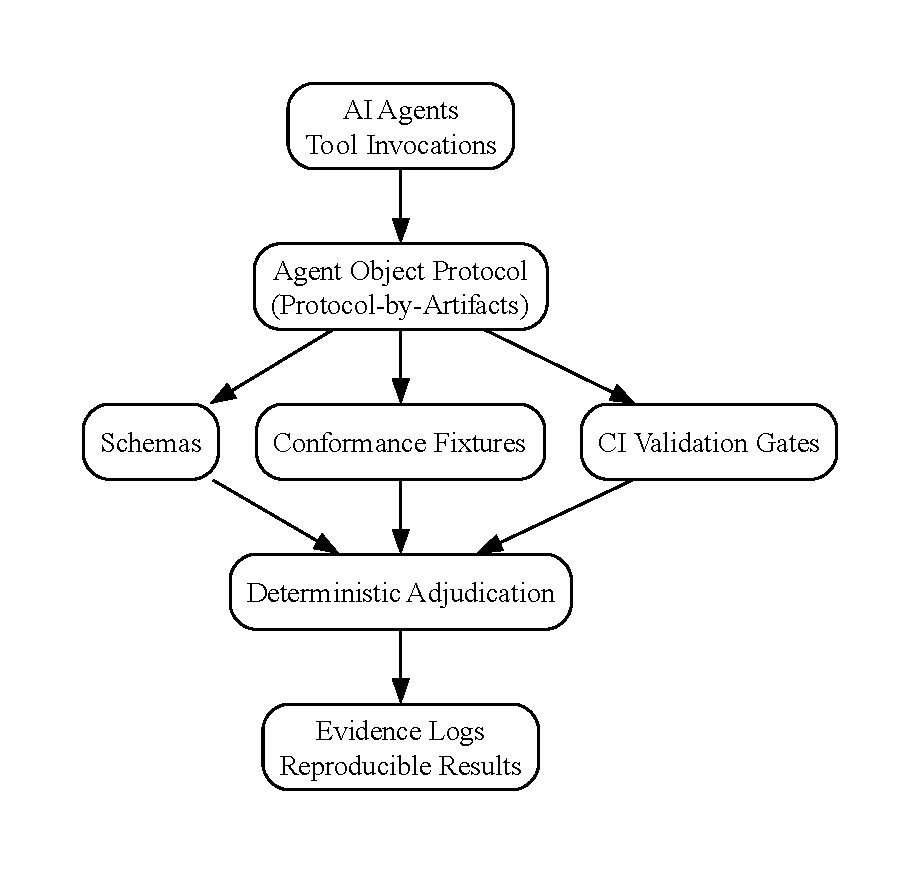
\includegraphics[width=0.9\linewidth]{figures/aop_architecture.pdf}
\caption{Architecture of the Agent Object Protocol (AOP). Protocol specifications are transformed into executable artifacts (schemas, fixtures, and CI validation gates) enabling deterministic adjudication of AI agent artifacts.}
\label{fig:aop_architecture}
\end{figure}


Figure~\ref{fig:aop_architecture} illustrates the AOP execution model. Agent
outputs are interpreted as protocol artifacts and routed through adjudication
components rather than directly to execution paths. This architecture separates
business function from protocol safety: tool execution is downstream of
admissibility, not a substitute for it.

The architecture also makes evidence first-class. Each gate emits
machine-readable outcomes that can be replayed or audited independently.
As a result, interoperability decisions become traceable artifacts, reducing
ambiguity during incident review or cross-organization verification.

\section{Evaluation}

We structure evaluation with five research questions:
\begin{itemize}
\item \textbf{RQ1}: Is parse-only validation sufficient for protocol
      adjudication?
\item \textbf{RQ2}: Are adjudication outcomes deterministic under repeated
      execution?
\item \textbf{RQ3}: Does AOP reject adversarial invalid artifacts reliably?
\item \textbf{RQ4}: Do AOP checks preserve classification fidelity at larger
      artifact scale?
\item \textbf{RQ5}: Are AOP outcomes consistent across independent validator
      implementations?
\end{itemize}

\subsection{Experimental Setup}

\begin{table}[t]
\centering
\caption{Experimental setup used across RQ1--RQ5.}
\begin{tabular}{@{}p{0.26\linewidth}p{0.68\linewidth}@{}}
\toprule
Component & Configuration \\
\midrule
Artifact corpus & 139 JSON artifacts (examples tree) \\
Scale corpus & 1000 synthetic artifacts (900 valid, 100 invalid) \\
Baseline script & \texttt{experiments/.../run\_benchmark.js} \\
Determinism script & \texttt{experiments/.../run\_ci\_test.sh} \\
Adversarial check & \texttt{validate\_invalid\_fixtures.mjs} \\
Scale script & \texttt{run\_synthetic\_scale.js} \\
Cross-validator script & \texttt{run\_cross\_validator.sh} \\
Execution mode & Scripted local/CI replay \\
Outputs & Text logs in experiment result files \\
\bottomrule
\end{tabular}
\end{table}

The setup intentionally uses lightweight scripts to reduce hidden
infrastructure assumptions. This design improves external reproducibility:
reviewers and practitioners can replay the same logic without custom
or proprietary tooling.

\subsection{Results Summary}

\begin{table}[t]
\centering
\caption{Evaluation summary for RQ1--RQ5.}
\begin{tabular}{lll}
\toprule
Experiment & Metric & Result \\
\midrule
Schema baseline & Parse rejection & 0/139 \\
Determinism & CI runs consistency & identical \\
Adversarial tests & Invalid rejection & 3/3 \\
Synthetic scale & Checks rejection / admission & 100/1000, 900/1000 \\
Cross-validator & Node/Python consistency & identical \\
\bottomrule
\end{tabular}
\end{table}

\begin{figure}[t]
\centering
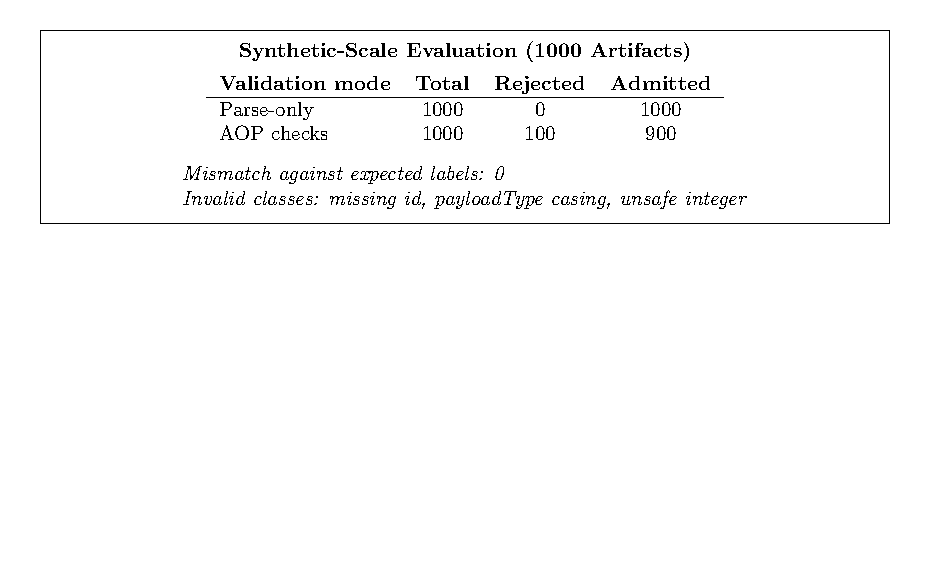
\includegraphics[width=0.95\linewidth]{figures/eval_scaling.pdf}
\caption{Evaluation scaling view. Parse-only validation rejects none of the 1000 synthetic artifacts, while AOP checks reject the 100 invalid samples and admit 900 valid samples with zero mismatch.}
\label{fig:eval_scaling}
\end{figure}


\subsection{RQ1: Parse-Only Sufficiency}

RQ1 is answered negatively. The parse-only baseline rejects none of the
139 artifacts, demonstrating that syntax acceptance is not a meaningful
adjudication boundary for protocol conformance. In particular,
duplicate-key ambiguity is not reliably surfaced by permissive parsing,
which can yield implementation-dependent interpretation.

\subsection{RQ2: Deterministic Replay}

RQ2 is answered positively for the tested setup. Repeated deterministic runs
produce identical adjudication summaries across three executions. This
stability supports replay-based auditing and makes gate outcomes dependable
for CI policy enforcement.

\subsection{RQ3: Adversarial Rejection}

RQ3 is also answered positively for the evaluated adversarial suite.
All three crafted invalid artifacts are rejected, with one parse-stage
rejection and two checks-stage rejections, and no unexpected pass. This
indicates that AOP captures both syntactic and semantic attack surfaces
within the adjudication pipeline.

\subsection{RQ4: Scale Stress Test}

RQ4 is answered positively on the synthetic-scale benchmark. We generated
1000 deterministic artifacts (900 valid, 100 invalid) and evaluated them with
both parse-only and AOP checks. Parse-only validation rejected 0 artifacts,
while AOP checks rejected exactly the 100 invalid samples and admitted 900
valid samples, with zero mismatch against expected labels.

This result does not claim full real-world representativeness; rather, it
shows that adjudication logic scales beyond the small handcrafted suite
without drift in classification behavior. The stress test therefore strengthens
internal validity for the protocol-by-artifacts decision boundary.

\subsection{RQ5: Cross-Implementation Consistency}

RQ5 is answered positively on the same 1000-artifact synthetic corpus. We run
two independently implemented validators (Node.js and Python) with equivalent
adjudication criteria and compare stage-level counts. Both implementations
report identical totals: 0 parse rejections, 100 checks rejections, and
900 admissions.

This result reduces the risk that reported behavior is an artifact of a single
runtime implementation. It also strengthens portability claims for AOP-style
adjudication when teams use different language stacks in production systems.

\subsection{Synthetic Failure-Class Breakdown}

To characterize rejection behavior on the scale corpus, we group invalid
synthetic artifacts into three classes: missing required identity fields
($n=50$), non-canonical payload-type casing ($n=30$), and unsafe integers
($n=20$). AOP checks reject all three classes with no false admission.

\begin{table}[t]
\centering
\caption{Class-level outcomes on the 1000-artifact synthetic corpus.}
\begin{tabular}{lcc}
\toprule
Invalid class & Count & Rejected \\
\midrule
Missing required \texttt{id} & 50 & 50 \\
Payload-type case confusion & 30 & 30 \\
Unsafe integer values & 20 & 20 \\
\bottomrule
\end{tabular}
\end{table}

\subsection{Runtime Snapshot}

We also measure lightweight runtime cost for replayability in constrained
review settings. On the evaluation environment, the parse baseline over the
139-artifact corpus completes in under 0.1s, while synthetic-scale generation
plus adjudication for 1000 artifacts completes in under 0.2s. Although these
numbers are not throughput benchmarks, they indicate that artifact-level
adjudication can be exercised quickly enough for reviewer-oriented replication
loops.

\subsection{Validity Considerations}

\textbf{Internal validity.} The synthetic-scale corpus is programmatically
generated and therefore may under-represent naturally occurring artifact noise.
To mitigate this, we include three distinct invalid classes mapped to observed
protocol failure modes (missing identity fields, payload-type confusion, and
unsafe numbers) and cross-check expected labels against adjudication outcomes.

\textbf{Construct validity.} Our core construct is machine-adjudicable
interoperability, operationalized as deterministic PASS/FAIL gate outcomes plus
replayable logs. This construct is narrower than full runtime correctness.
An artifact that passes protocol gates may still fail during downstream business
execution, but such failures are intentionally out of scope for conformance
adjudication.

\textbf{External validity.} The evaluation currently uses one repository corpus
and one synthetic benchmark, with two validator implementations over the
synthetic corpus. Results should therefore be interpreted as evidence of
feasibility and consistency, not as universal performance claims across all
agent ecosystems. Future replication should include additional independent
implementations and broader domain-specific corpora.

\textbf{Conclusion validity.} Determinism claims are based on repeated
script-level replay and stable summaries over three runs. While this supports
consistency under the tested toolchain, stronger statistical confidence would
benefit from larger repetition counts and controlled environment perturbations.

\subsection{Synthesis Across RQ1--RQ5}

Taken together, the five research questions characterize a layered argument for
artifact-first protocol engineering. RQ1 establishes that parse acceptance is an
inadequate proxy for protocol correctness. RQ2 and RQ3 show that adjudication
logic is both stable under replay and effective against targeted adversarial
inputs. RQ4 extends this claim to larger corpus volume without label drift, and
RQ5 adds cross-implementation evidence that outcomes are not tied to a single
runtime stack.

This progression is methodologically important for ICSE-style evaluation. Many
interoperability papers focus on one axis (for example, parser strictness or
throughput) and leave external replay behavior implicit. Our design instead
connects sufficiency, determinism, security rejection, scaling, and portability
within one executable pipeline. The result is a tighter link between claims and
evidence artifacts.

The synthesis also clarifies scope. We do not claim that AOP solves all aspects
of software integration quality. Rather, we claim that AOP provides a robust
adjudication substrate for deciding protocol admissibility before execution.
This narrower claim is directly testable and reproducible, which is a practical
advantage for both engineering teams and artifact-focused peer review.

\section{Case Study: Tool Protocol Validation}

To demonstrate practical applicability, we evaluate AOP on a simplified
tool invocation workflow representative of production agent-tool systems.
The case study focuses on protocol adjudication quality, not tool business
logic, and therefore isolates validation behavior from downstream execution.

\subsection{Scenario and Workflow}

In modern AI agent stacks, an invocation lifecycle often follows four steps:
\begin{enumerate}
\item The agent emits an invocation artifact.
\item A validator checks structural and policy-level conformance.
\item The tool runtime executes only if validation passes.
\item Outputs and evidence are persisted for replay and audit.
\end{enumerate}

In many deployments, step (2) is implemented as parse-only schema checks.
AOP augments this stage with fixture-aware and gate-aware adjudication.
\begin{figure}[t]
\centering
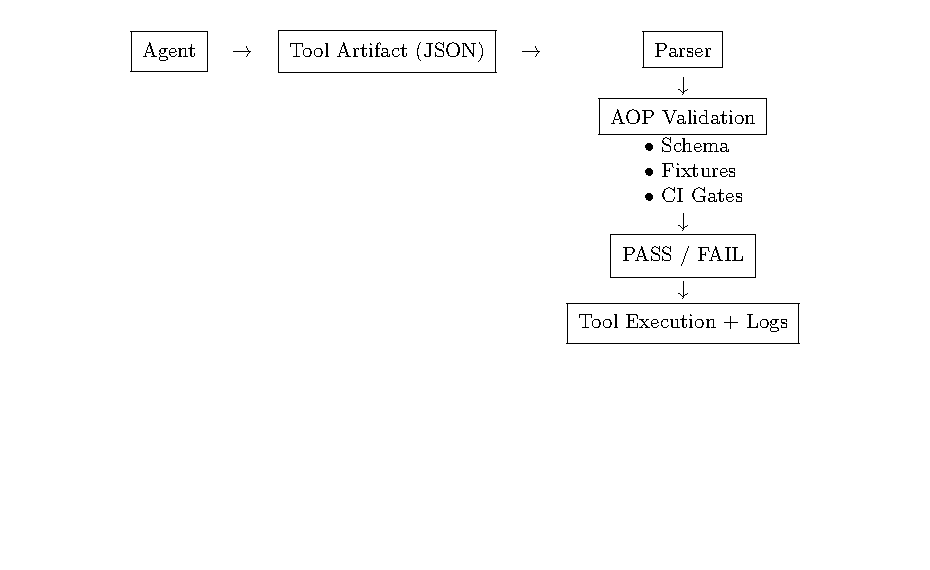
\includegraphics[width=0.9\linewidth]{figures/tool_protocol_flow.pdf}
\caption{Tool invocation workflow evaluated in the case study. Artifacts produced by AI agents are validated through AOP schema, fixtures, and CI adjudication gates.}
\label{fig:tool_protocol}
\end{figure}


\subsection{Concrete Protocol Instance}

To ground the case study in a concrete protocol shape, we use the
tool-invocation artifact below as a representative valid request:
\begin{quote}
\ttfamily
\{\\
\ \ "aop\_version": "1.0",\\
\ \ "kind": "tool\_invocation",\\
\ \ "id": "req-1042",\\
\ \ "tool": \{"name": "battery\_status",\\
\ \ \ \ "arguments": \{"asset\_id": "A-77"\}\},\\
\ \ "envelope": \{"payloadType":\\
\ \ \ \ "application/vnd.in-toto+json"\}\\
\}
\end{quote}

This artifact class is common in agent-tool ecosystems: a caller provides a
tool identifier, structured arguments, and an evidence envelope pointer.
Case-study invalid samples mutate this shape by removing required identity
fields, altering payload-type casing, or introducing unsafe numeric content.

\subsection{Artifacts and Data}

The case study uses the repository's executable artifact set, including
valid examples, negative fixtures, and adversarial invalid inputs.
The benchmark corpus size is 139 artifacts, and adversarial samples include
duplicate-key ambiguity, non-canonical in-toto payload type casing, and
unsafe integer edge values.

To keep the study reproducible, all checks are executed via scriptable
pipelines rather than manual inspection. This allows direct replay in CI
and local environments using identical commands and fixture directories.

\subsection{Baseline: Parse-Only Validation}

The baseline validator applies parse-level checks and schema loading without
semantic adjudication. This mirrors common minimal validation in real systems
where ``valid JSON'' is treated as sufficient precondition for execution.

In this setup, artifacts with semantic inconsistencies can still pass initial
validation if their syntax is accepted. Duplicate-key ambiguity is a canonical
example: permissive parsers often collapse repeated keys rather than rejecting
the artifact, creating non-portable interpretation risk across runtimes.

\subsection{AOP Validation Pipeline}

AOP validates artifacts through three deterministic layers:
\begin{itemize}
\item \textbf{Schema validation}: required fields, type constraints,
      and closed-world shape checks.
\item \textbf{Conformance fixtures}: positive and negative fixture outcomes
      encoded as executable expectations.
\item \textbf{CI adjudication gates}: automated PASS/FAIL gate decisions
      producing replayable logs.
\end{itemize}

An artifact must pass all layers to be admitted for execution.
If a gate fails, the artifact is rejected with explicit failure mode
classification (parse-stage or checks-stage), improving triage precision.

\subsection{Operational Results}

\begin{table}[t]
\centering
\caption{Case study outcomes on tool protocol artifacts.}
\begin{tabular}{lll}
\toprule
Stage & Metric & Outcome \\
\midrule
Baseline parse-only & Rejected artifacts & 0 / 139 \\
AOP determinism & Repeatability (3 runs) & identical \\
AOP adversarial gate & Rejected invalid cases & 3 / 3 \\
\bottomrule
\end{tabular}
\end{table}

The baseline confirms that parse-only acceptance is not an adjudication
criterion. Under AOP, repeated runs produce stable outputs, and adversarial
samples are deterministically rejected with no unexpected pass.

\subsection{Case Study Implications}

This case shows that protocol-by-artifacts is directly deployable in tool
invocation workflows without coupling to a specific runtime implementation.
The key operational gain is predictable gate behavior: teams can reason
about admissibility using replayable evidence instead of ad hoc parser
semantics.

The same structure can be extended to additional domains (policy decisions,
registry exchanges, and evidence envelopes) by adding fixture families and
gate checks while preserving the adjudication model.


\section{Threat Model}

We consider adversarial attempts to bypass admissibility before tool execution.
The threat model emphasizes artifact-level attacks, where malicious or malformed
inputs exploit parser behavior, schema blind spots, or evidence mutation.

\begin{table}[t]
\centering
\caption{Threat classes and AOP detection points.}
\begin{tabular}{lll}
\toprule
Attack class & Example & Detection layer \\
\midrule
Parser ambiguity & Duplicate JSON keys & Parse/strict decode \\
Payload confusion & Invalid payload semantics & Check stage \\
Tampered artifacts & Mutated evidence or fixtures & Fixture/gate stage \\
\bottomrule
\end{tabular}
\end{table}

AOP assumes an honest execution substrate for running checks, but does not
assume honest input producers. The primary defensive strategy is deterministic
rejection before execution, coupled with replayable gate evidence.

\section{Related Work}

\subsection{Schema-First Contracts and Interface Validation}

Schema-centric approaches remain a practical first line for protocol quality.
Canonicalization guidance such as RFC 8785~\cite{rfc8785} and interface-level
tool contracts such as MCP~\cite{mcp_tools_20250618} reduce ambiguity in field
representation, naming, and transport-level interoperability. However, schema-
first workflows usually answer only one question: whether an artifact can be
structurally accepted. They do not fully define adjudication semantics for
negative fixtures, parser ambiguity, or policy-gated admission decisions.

This distinction is central to our positioning. AOP keeps schema validation as
an entry gate but treats it as necessary rather than sufficient. The remaining
adjudication stages (fixtures, semantic checks, and CI gates) resolve questions
that schema-only acceptance cannot answer consistently across implementations.

\subsection{Attestation and Provenance Systems}

Attestation ecosystems contribute critical evidence primitives. In-toto envelope
formats~\cite{intoto_envelope_v1} provide portable signed claim containers, and
SLSA provenance guidance~\cite{slsa_prov_v11} formalizes stronger traceability
expectations for build and release processes. These mechanisms are highly
relevant for integrity of artifacts and lineage records.

Yet provenance and adjudication solve different problems. Provenance asks
``where did this artifact come from and can we trust its chain of custody?''
Adjudication asks ``does this artifact satisfy protocol intent and safety
constraints under explicit gate policies?'' AOP focuses on the latter while
remaining compatible with provenance-oriented evidence envelopes.

\subsection{Reproducibility and Artifact Evaluation in SE}

Recent software engineering practice places increasing weight on reproducibility
and artifact availability~\cite{acm_artifact_badging_2020,
icse_open_science_2027}. At the same time, meta-analysis reports that many
published artifacts remain difficult to exercise or reproduce in independent
settings~\cite{icse_artifact_state_2026}. This gap motivates evaluation models
that minimize hidden assumptions and make acceptance criteria machine-checkable.

AOP aligns with this direction by expressing conformance claims as replayable
checks and stage-level logs instead of prose-only statements. In this sense, it
is not only a protocol design method but also an artifact-evaluation method
that links research claims to executable adjudication outputs.

\subsection{Protocol Governance and Evolution}

A recurring challenge in protocol ecosystems is governance drift: implementations
evolve at different speeds, while textual specifications lag behind operational
reality. Most prior work addresses this through versioning conventions and API
compatibility advice; fewer approaches define explicit, executable criteria for
when a change is admission-safe versus breaking.

AOP contributes a governance-oriented mechanism by binding protocol evolution to
fixture deltas and gate outcomes. Under this model, introducing a new rule is
not only a textual update but an executable change in adjudication behavior.
This improves reviewability for both maintainers and external evaluators.

\subsection{Comparative Positioning}

\begin{table}[t]
\centering
\caption{Positioning of AOP relative to adjacent approaches.}
{\small
\setlength{\tabcolsep}{3pt}
\begin{tabular}{@{}p{0.27\linewidth}p{0.20\linewidth}p{0.22\linewidth}p{0.23\linewidth}@{}}
\toprule
Approach family & Structural validation & Deterministic adjudication & Replay-ready evidence \\
\midrule
Schema-first contracts & Strong & Limited & Limited \\
Provenance systems & Indirect & Limited & Strong \\
Artifact badging workflows & Indirect & Indirect & Medium \\
AOP (this work) & Strong & Strong & Strong \\
\bottomrule
\end{tabular}
}
\end{table}

The table summarizes why AOP is complementary rather than competing with prior
work. It combines structural checks, deterministic decision semantics, and
replay-ready outputs in one executable contract, which is the core design goal
for machine-adjudicable protocol interoperability.

\section{Implementation and Reproducibility Protocol}

\subsection{Reference Validation Workflow}

The reference workflow is implemented as a script-composed pipeline that
separates three concerns: corpus scanning, deterministic validation, and gate
materialization. Corpus scanning measures parse-stage behavior over the
artifact set. Deterministic validation executes strict checks and fixture
expectations. Gate materialization emits replayable summaries and stage-level
rejection counts. This decomposition allows each stage to be independently
audited while preserving end-to-end reproducibility.

The practical benefit of this workflow is failure localization. When a fixture
is rejected, logs identify whether failure occurred during parse, during
semantic checks, or at policy gate evaluation. This enables developers to
distinguish malformed inputs from rule regressions and policy mismatches.

\subsection{Gate Taxonomy}

\begin{table}[t]
\centering
\caption{AOP gate taxonomy used in the implementation workflow.}
{\small
\setlength{\tabcolsep}{3pt}
\begin{tabular}{@{}p{0.15\linewidth}p{0.23\linewidth}p{0.52\linewidth}@{}}
\toprule
Gate type & Scope & Output artifact \\
\midrule
Parse gate & JSON decoding and ambiguity checks & Parse rejection log \\
Schema gate & Shape/type constraints & Schema report \\
Fixture gate & Expected pass/fail & Fixture summary \\
Semantic gate & Protocol-specific invariants & Check-stage failure detail \\
CI gate & Admission policy & PASS/FAIL record \\
\bottomrule
\end{tabular}
}
\end{table}

The taxonomy clarifies why parse-only systems are incomplete. Parse and schema
gates can ensure structural admissibility, but fixture and semantic gates are
required to enforce protocol intent under adversarial or edge-case inputs.

\subsection{Replay Procedure}

Reproducibility is operationalized through a fixed command sequence and
deterministic result files:
\begin{itemize}
\item \path{./experiments/run_all.sh}
\item \path{cat experiments/schema-benchmark/results/benchmark.txt}
\item \path{cat experiments/ci-determinism/results.txt}
\item \path{cat experiments/adversarial-tests/results.txt}
\item \path{cat experiments/synthetic-scale/results/results.txt}
\item \path{cat experiments/cross-validator/results/results.txt}
\end{itemize}

To support third-party verification, expected invariants are checked at five
levels: baseline parse rejection count, cross-run determinism equality,
adversarial unexpected-pass count, synthetic-scale mismatch count, and
cross-validator equality between Node and Python summaries. This enables
reviewers to validate claims without relying on hidden infrastructure
assumptions.

\subsection{Cross-Validator Harness Design}

The cross-validator experiment is intentionally implemented with independent
Node and Python scripts that mirror adjudication rules but do not share parser
internals or helper libraries. This separation avoids ``same-code duplicated''
bias and creates a stronger portability check for gate logic. The harness then
normalizes outputs to stage-level counts (total, parse-rejected, checks-
rejected, admitted) and performs strict equality checks before reporting a
consistency verdict.

Two design choices improve maintainability. First, the harness consumes the
same generated corpus used in RQ4, preventing hidden sampling differences
between implementations. Second, the summary format is line-oriented plain text
so that CI jobs and reviewers can inspect diffs without custom parsers.
Although simple, this design makes cross-runtime parity auditable in routine
pull-request workflows.

\subsection{Reviewer-Oriented Replication Checklist}

For artifact-oriented evaluation, we use a concise replication checklist:
\begin{enumerate}
\item Confirm that scripts execute without manual patching.
\item Verify that corpus size and baseline metrics match the paper.
\item Compare deterministic run outputs for equality across repetitions.
\item Validate that adversarial fixtures produce zero unexpected pass.
\item Confirm that synthetic-scale results report 1000 artifacts and zero mismatch.
\item Confirm that cross-validator results report \texttt{Consistent: true}.
\item Inspect generated logs for stage-level failure classification.
\end{enumerate}

This checklist is intended to reduce replication ambiguity and align practical
review workflows with adjudication-centric protocol claims.

\section{Discussion}

\subsection{Artifact Evaluation Readiness}

The artifact package is organized for documented, consistent, complete, and
exercisable evaluation:

\begin{verbatim}
experiments/
  run_all.sh
  schema-benchmark/
  ci-determinism/
  adversarial-tests/
  synthetic-scale/
  cross-validator/
\end{verbatim}

This layout reduces reviewer setup overhead and supports direct replay of the
reported results.

\subsection{Practical Implications}

For practitioners, protocol-by-artifacts shifts conformance enforcement left
into CI, reducing reliance on late-stage integration debugging. For reviewers
and auditors, deterministic gate logs provide clearer evidence chains than
informal schema claims.

\subsection{Generalization Boundaries}

The present evaluation supports feasibility across two axes: corpus diversity
(repository artifacts plus synthetic stress data) and implementation diversity
(Node and Python validators). However, several boundaries remain. First, the
artifacts largely target JSON-centric interfaces and may not capture binary or
streaming protocol idioms. Second, the tested governance policy is single-
pipeline and does not model federated policy conflicts between organizations.

These boundaries suggest a practical interpretation: AOP currently demonstrates
strong internal reproducibility for artifact-first protocol workflows, while
full ecosystem generalization requires additional cross-domain replications.
Future studies should include event-stream protocols, multi-tenant policy sets,
and validator heterogeneity beyond two language runtimes.

\subsection{Protocol Governance and Standardization Path}

For long-term sustainability, protocol-by-artifacts requires governance practices
that treat fixtures and gate policies as first-class normative material. We
outline a minimal governance path with three layers:
\begin{enumerate}
\item \textbf{Normative core}: frozen schema constraints and mandatory negative
      fixtures required for conformance.
\item \textbf{Profile layer}: optional policy profiles for domain-specific
      admissibility criteria.
\item \textbf{Change control}: versioned gate deltas reviewed through reproducible
      replay before adoption.
\end{enumerate}

This structure can reduce ambiguity during protocol evolution. Instead of
debating solely from prose, maintainers can inspect concrete fixture deltas and
their effect on PASS/FAIL boundaries, then decide whether a change is minor,
profile-scoped, or breaking at the protocol core.

\subsection{Archival and Evaluation Readiness}

For conference artifact review, reproducibility requires more than executable
scripts: it also requires stable packaging and long-term referenceability.
In line with open-science guidance~\cite{icse_open_science_2027}, a practical
submission package should include: (1) an immutable archive snapshot, (2) a
minimal replay guide with expected outputs, and (3) explicit environment
assumptions for validator execution. AOP aligns naturally with this requirement
because gate outcomes are already produced as deterministic text artifacts.

This packaging view also helps bridge paper review and artifact review. The
paper can report high-level claims and RQ outcomes, while archived artifacts
provide executable evidence for each claim boundary. Maintaining this claim-to-
artifact linkage reduces ambiguity during rebuttal and post-acceptance
verification.

\subsection{Adoption Risks}

Artifact-first adjudication also introduces practical risks. Teams may overfit
to published fixtures, creating ``teaching to the test'' dynamics where unseen
edge cases remain weakly protected. There is also operational risk if CI gate
policies become too strict for early-stage integrations, causing high friction
and delayed adoption.

Mitigations include rotating adversarial fixture sets, maintaining explicit
policy tiers (warning vs blocking gates), and documenting migration windows for
breaking changes. These safeguards preserve the core benefit of deterministic
adjudication while keeping integration pathways realistic for evolving systems.

\subsection{Limitations and Future Work}

Current evaluation combines one real repository corpus and one synthetic-scale
dataset; both remain narrower than multi-organization production traffic.
Future work should broaden adversarial diversity, evaluate multi-language
validator parity, and measure performance overhead under larger and noisier
artifact volumes. A larger cross-ecosystem case study would further validate
external generalizability.

\section{Conclusion}

AOP operationalizes machine-adjudicable interoperability via executable
protocol artifacts. Across baseline, determinism, and adversarial experiments,
results show that parse-only validation is insufficient, while deterministic
gate-based adjudication provides stronger and reproducible conformance
behavior. The case study demonstrates integration feasibility in tool protocol
workflows, and the artifact package supports replay-oriented evaluation for
future research and deployment.

\bibliographystyle{IEEEtran}
\bibliography{refs}

\end{document}
